\documentclass{article}

\usepackage[latin1]{inputenc}
\usepackage{amsmath}
\usepackage{amsfonts}
\usepackage{amssymb}
\usepackage{array}
\usepackage{parskip}
\usepackage{graphicx}
%\usepackage{dsfont}
\usepackage{framed}
\usepackage{ upgreek }
\usepackage{listings}
\lstset{frame=single}
\lstset{basicstyle=\small}
\usepackage{fancyhdr}
\setlength{\headheight}{15.2pt}
\pagestyle{fancy}
\setlength{\parindent}{0pt}
\setcounter{secnumdepth}{2}
\usepackage{graphicx}
\usepackage{float}

%\usepackage{sectsty}

\begin{document}

% title stuff
\title{Interactive Fractal Viewer \\
CSEE W4840 Project Design}
\author{Nathan Hwang - nyh2105@columbia.edu \and
Richard Nwaobasi - rcn2105@columbia.edu \and
Luis Pe\~{n}a - lep2141@columbia.edu \and
Stephen Pratt - sdp2128@columbia.edu }

\maketitle
\newpage
\abstract{Fractals are often appreciated for their rich and elegant
  internal complexity. This complexity is responsible for the
  beautiful aesthetic of these famed mathematical images as well as
  the amount of computational power required to generate them. Using
  fixed point calculations within parallelized sequential logic
  blocks, we aim to develop an hardware-accelerated fractal generator,
  capable of computing and displaying quadratic Julia sets in
  significantly less time than a software-based solution.}

% ------------------------------------------------------------
% and we begin the design document proper


% ------------------------------------------------------------
\section{High-level Overview}

The following is a description the high-level block structure of the project:

\begin{itemize}
\item The UI Module is responsible for reading user input, translating
  that input into information relevant to the remainder of the system,
  and communicating the results.
\item A Window Generator builds a set of 4-tuples $(x, y, a, b)$ where
  each tuple is a mapping from a VGA coordinate $(x, y)$ to a value in
  the complex plane of the form $a+bi$.
\item Given a complex number specified by the ordered pair $(a, b)$,
  components known as Iterative Function Modules the number of
  function iterations required for a specified value to become
  unbounded. Multiple IFMs work in parallel.

\item These tuples are requested systematically by a component known
  as the Parallel


\item The processor writes its values across its bus into a queue,
  which feeds values to Iterative Function Modules (IFMs).

\item Another queue recieves 3-tuples $(x, y, c)$ from the IFMs, where
  $(x, y)$ corresponds to a VGA coordinate and $c$ is the breakaway
  constant computed by the IFM. These values are passed one at a time
  to a buffer known as the Coordinate-Breakaway Lookup Table.
\item The VGA module fetches results from the Coordinate-Breakaway
  Lookup Table and colorizes them using a separate RAM-based lookup
  table, displaying the result.
\end{itemize}

These encompass only the so called ``critical modules'', what is
absolutely needed to have a fast draw of the fractal. Further work,
known as parameterization modules, offer various ways to mutate the
parameters used to draw the fractal.

\newpage

\begin{figure}[H]
  \centering
	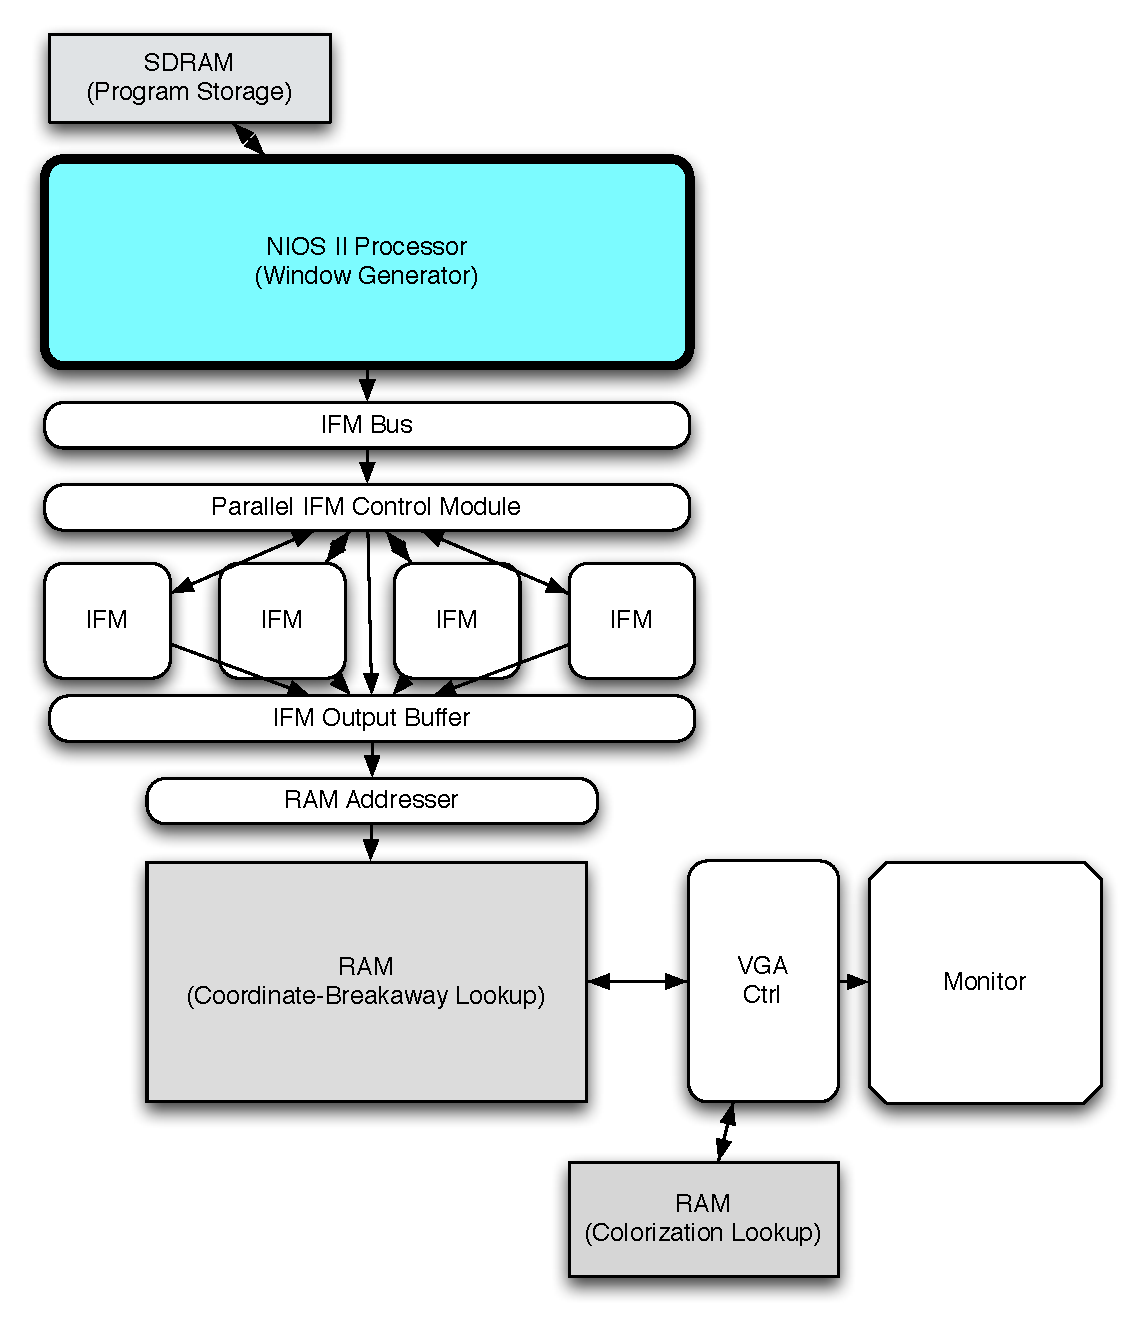
\includegraphics[width=\textwidth]{block_diagrams/top_level.pdf}
  \caption{High-level Block Diagram}
\end{figure}
\newpage

% ------------------------------------------------------------
% now, we delve into the lower levels of the implementation
% ------------------------------------------------------------
\section{Critical Modules}

% ----------------------------------------
\subsection{UI Module}

As an interactive device, our fractal generator has the capacity to
accept user parameters such as window size or Julia set constants
during operation. This communication with the user is facilitated by
the UI module, which is implemented on the NIOS II processor. This
module is responsible for handling communication with input
peripherals and translating user input into information that can
easily be used by the hardware-based fractal generator. Once this
information has been translated into a set of instructions for the
generator, these instructions are written to a specialized bus across
the Avalon interconnect fabric.

\begin{figure}[H]
  \centering
    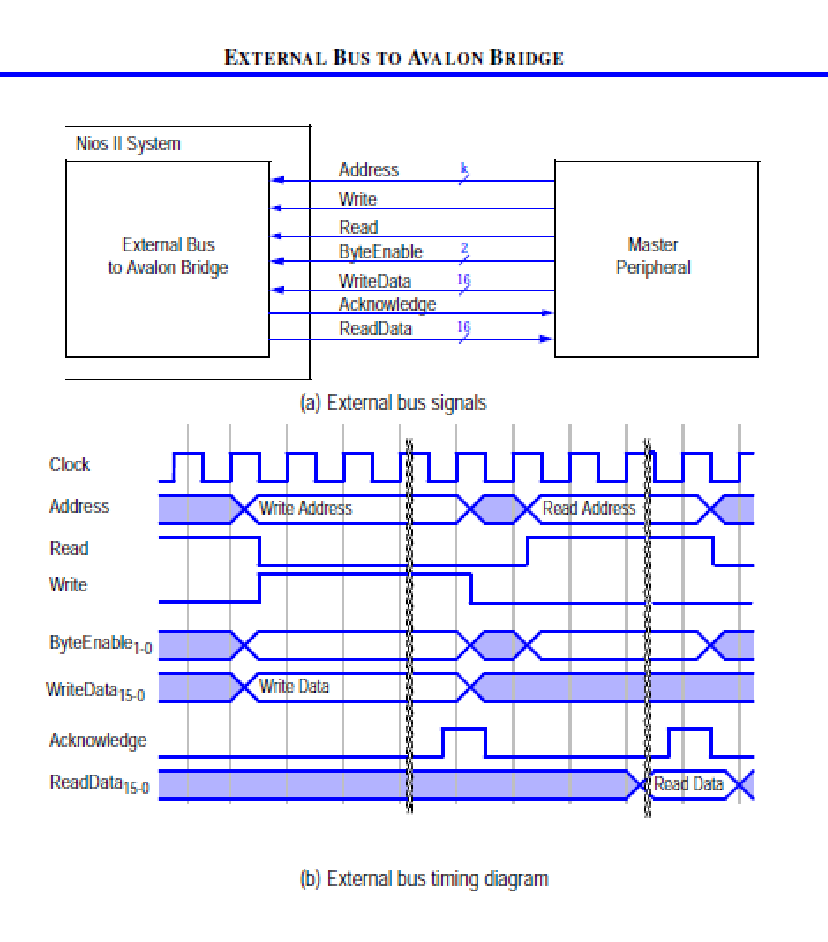
\includegraphics[width=200pt]{block_diagrams/nbat.pdf}
  \caption{Block and Timing Diagram of the Avalon interconnect
    fabric. Provided by Altera Corporation.}
\end{figure}

Parameters of primary concern are those of viewing window and Julia
set constant. The window is set using the following values (which will
be elaborated on in the next section)

\begin{itemize}
\item $a_{min} - 36$ bits
\item $a_{diff} - 36$ bits
\item $a_{leap} - 10$ bits
\item $b_{min} - 36$ bits
\item $b_{diff} - 36$ bits
\item $b_{leap} - 10$ bits
\end{itemize}

Meanwhile, the Julia set constant is set using the following values

\begin{itemize}
\item $c_{real} - 36$ bits
\item $c_{img} - 36$ bits
\end{itemize}

Because the Avalon interconnect fabric only allows for 32 bits of data
to be written at once, the UI module communicates with the bus using a
specialized protocol. In this protocol, the four least significant
bits of data transmitted indicate the nature of the data.


\begin{tabular}{| l | l | }\\ \hline
XXXXXXXXXXXXXX$|_{21}$AAAAAAAAAAAAAAAAAA$|_3$0000$|_0$ & $a_{min}$ (18 MSB)\\ \hline
XXXXXXXXXXXXXX$|_{21}$AAAAAAAAAAAAAAAAAA$|_3$0001$|_0$ & $a_{min}$ (18 LSB)\\\hline
XXXXXXXXXXXXXX$|_{21}$AAAAAAAAAAAAAAAAAA$|_3$0010$|_0$ & $a_{diff}$ (18 MSB)\\\hline
XXXXXXXXXXXXXX$|_{21}$AAAAAAAAAAAAAAAAAA$|_3$0011$|_0$ & $a_{diff}$ (18 LSB)\\\hline
XXXXXXXXXXXXXXXXXXXXXX$|_{12}$AAAAAAAAAA$|_3$0100$|_0$ & $a_{leap}$ \\\hline
XXXXXXXXXXXXXX$|_{21}$BBBBBBBBBBBBBBBBBB$|_3$0101$|_0$ & $b_{min}$ (18 MSB)\\\hline
XXXXXXXXXXXXXX$|_{21}$BBBBBBBBBBBBBBBBBB$|_3$0110$|_0$ & $b_{min}$ (18 LSB)\\\hline
XXXXXXXXXXXXXX$|_{21}$BBBBBBBBBBBBBBBBBB$|_3$0111$|_0$ & $b_{diff}$ (18 MSB)\\\hline
XXXXXXXXXXXXXX$|_{21}$BBBBBBBBBBBBBBBBBB$|_3$1000$|_0$ & $b_{diff}$ (18 LSB)\\\hline
XXXXXXXXXXXXXXXXXXXXXX$|_{12}$BBBBBBBBBB$|_3$0100$|_0$ & $a_{leap}$ \\\hline
XXXXXXXXXXXXXX$|_{21}$CCCCCCCCCCCCCCCCCC$|_3$1010$|_0$ & $c_{real}$ (18 MSB)\\\hline
XXXXXXXXXXXXXX$|_{21}$CCCCCCCCCCCCCCCCCC$|_3$1011$|_0$ & $c_{real}$ (18 LSB)\\\hline
XXXXXXXXXXXXXX$|_{21}$CCCCCCCCCCCCCCCCCC$|_3$1100$|_0$ & $c_{img}$ (18 MSB)\\\hline
XXXXXXXXXXXXXX$|_{21}$CCCCCCCCCCCCCCCCCC$|_3$1101$|_0$ & $c_{img}$ (18 LSB)\\\hline
XXXXXXXXXXXXXXXXXXXXXXXXXXXXXXXX$_3$1111 & End Transmission\\\hline
\end{tabular}

We have the Nios II configured to use the SDRAM as its memory store,
making the SRAM available for other uses.

\subsection{Window Generator}

The window generator serves to kick off the calculation cascade,
calculating the position of each pixel in the complex plane given the
input window, thereby producing $(x, y, a, b)$ tuples.

\begin{figure}[H]
  \centering
    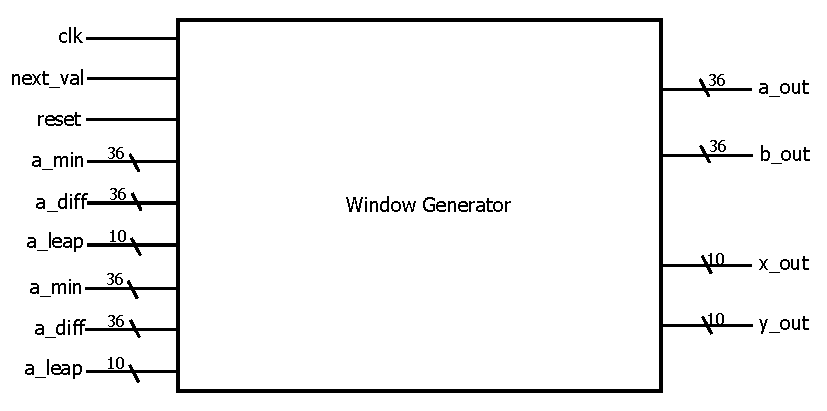
\includegraphics[width=160pt]{block_diagrams/win_gen.pdf}
  \caption{High-level Block Diagram of the Window Generator}
\end{figure}


The generator uses a specialized procedure that requires only addition
and comparison operations to map out a whole window. Say we have a
window that stretches from $v_{min}$ to $v_{max}$ over N pixels. The
procedure works by iterating from 0 to N-1 and producing a sum at each
step of the way that corresponds to a the value of $v$ at that
point. The procedure requires a few values as input:


\begin{itemize}
\item $a_{min} - 36$ bits: Describes the minimum value of $a$ in the window
\item $a_{diff} - 36$ bits: Describes the standard differential
  between consecutive a values in the window $(a_{max} -
  a_{min})/WIDTH_{SCREEN}$ this is computed by the NIOS processor.
\item $a_{leap} - 10$ bits: Periodically, we will need to add 1 to our
  sum to compensate for precision loss. This value corresponds to the
  length of the intervals between these "leap cycles"
  $WIDTH_{SCREEN}/((a_{max} - a_{min})\%WIDTH_{SCREEN})$
\item $b_{min} - 36$ bits: Describes the minimum value of $a$ in the window
\item $b_{diff} - 36$ bits: Describes the standard differential
  between consecutive a values in the window $(b_{max} -
  ab_{min})/HEIGHT_{SCREEN}$ this is computed by the NIOS processor.
\item $b_{leap} - 10$ bits: Periodically, we will need to add 1 to our
  sum to compensate for precision loss. This value corresponds to the
  length of the intervals between these "leap cycles"
  $HEIGHT_{SCREEN}/((b_{max} - b_{min})\%HEIGHT_{SCREEN})$
\end{itemize}

The window generator is therefore comprised of two "differential
counters" that are responsible for performing the iterations. One
computes values for $b$ and the other $a$.

\begin{figure}[h!]
  \centering
    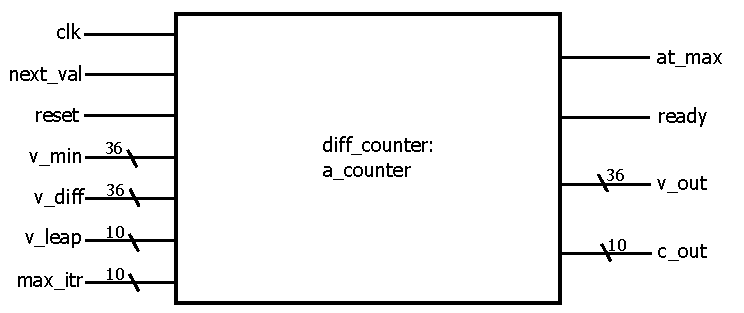
\includegraphics[width=160pt]{block_diagrams/acounter.pdf}
  \caption{Block diagram of a differential counter used in window generation}
\end{figure}

When the differential counter receives a reset signal, it initializes
its data according to the signals coming in.  Then, each time it
recieves a next-value signal, it increments the output value
accordingly. If the counter reaches its maximum, it asserts a flag.

\begin{figure}[H]
  \centering
    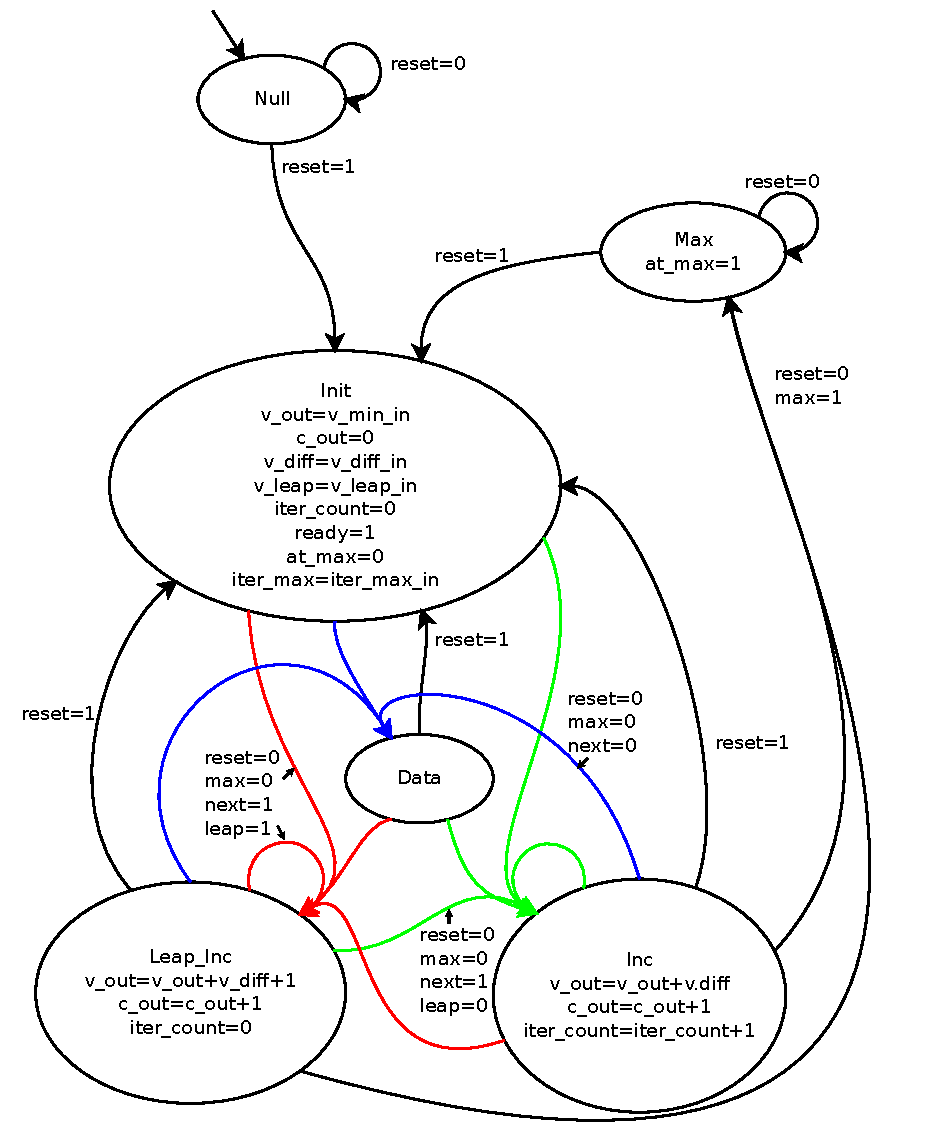
\includegraphics[width=200pt]{state_diagrams/diff_counter.pdf}
  \caption{State Diagram for the diff counter, Moore machine: signals
    \texttt{max=c\_cuis=max\_itr}, \texttt{leap=iter\_count=v\_leap}. Omit
    unused signals (X) for compactness. Colorcoded signal bundles.}
\end{figure}

\begin{figure}[H]
  \centering
    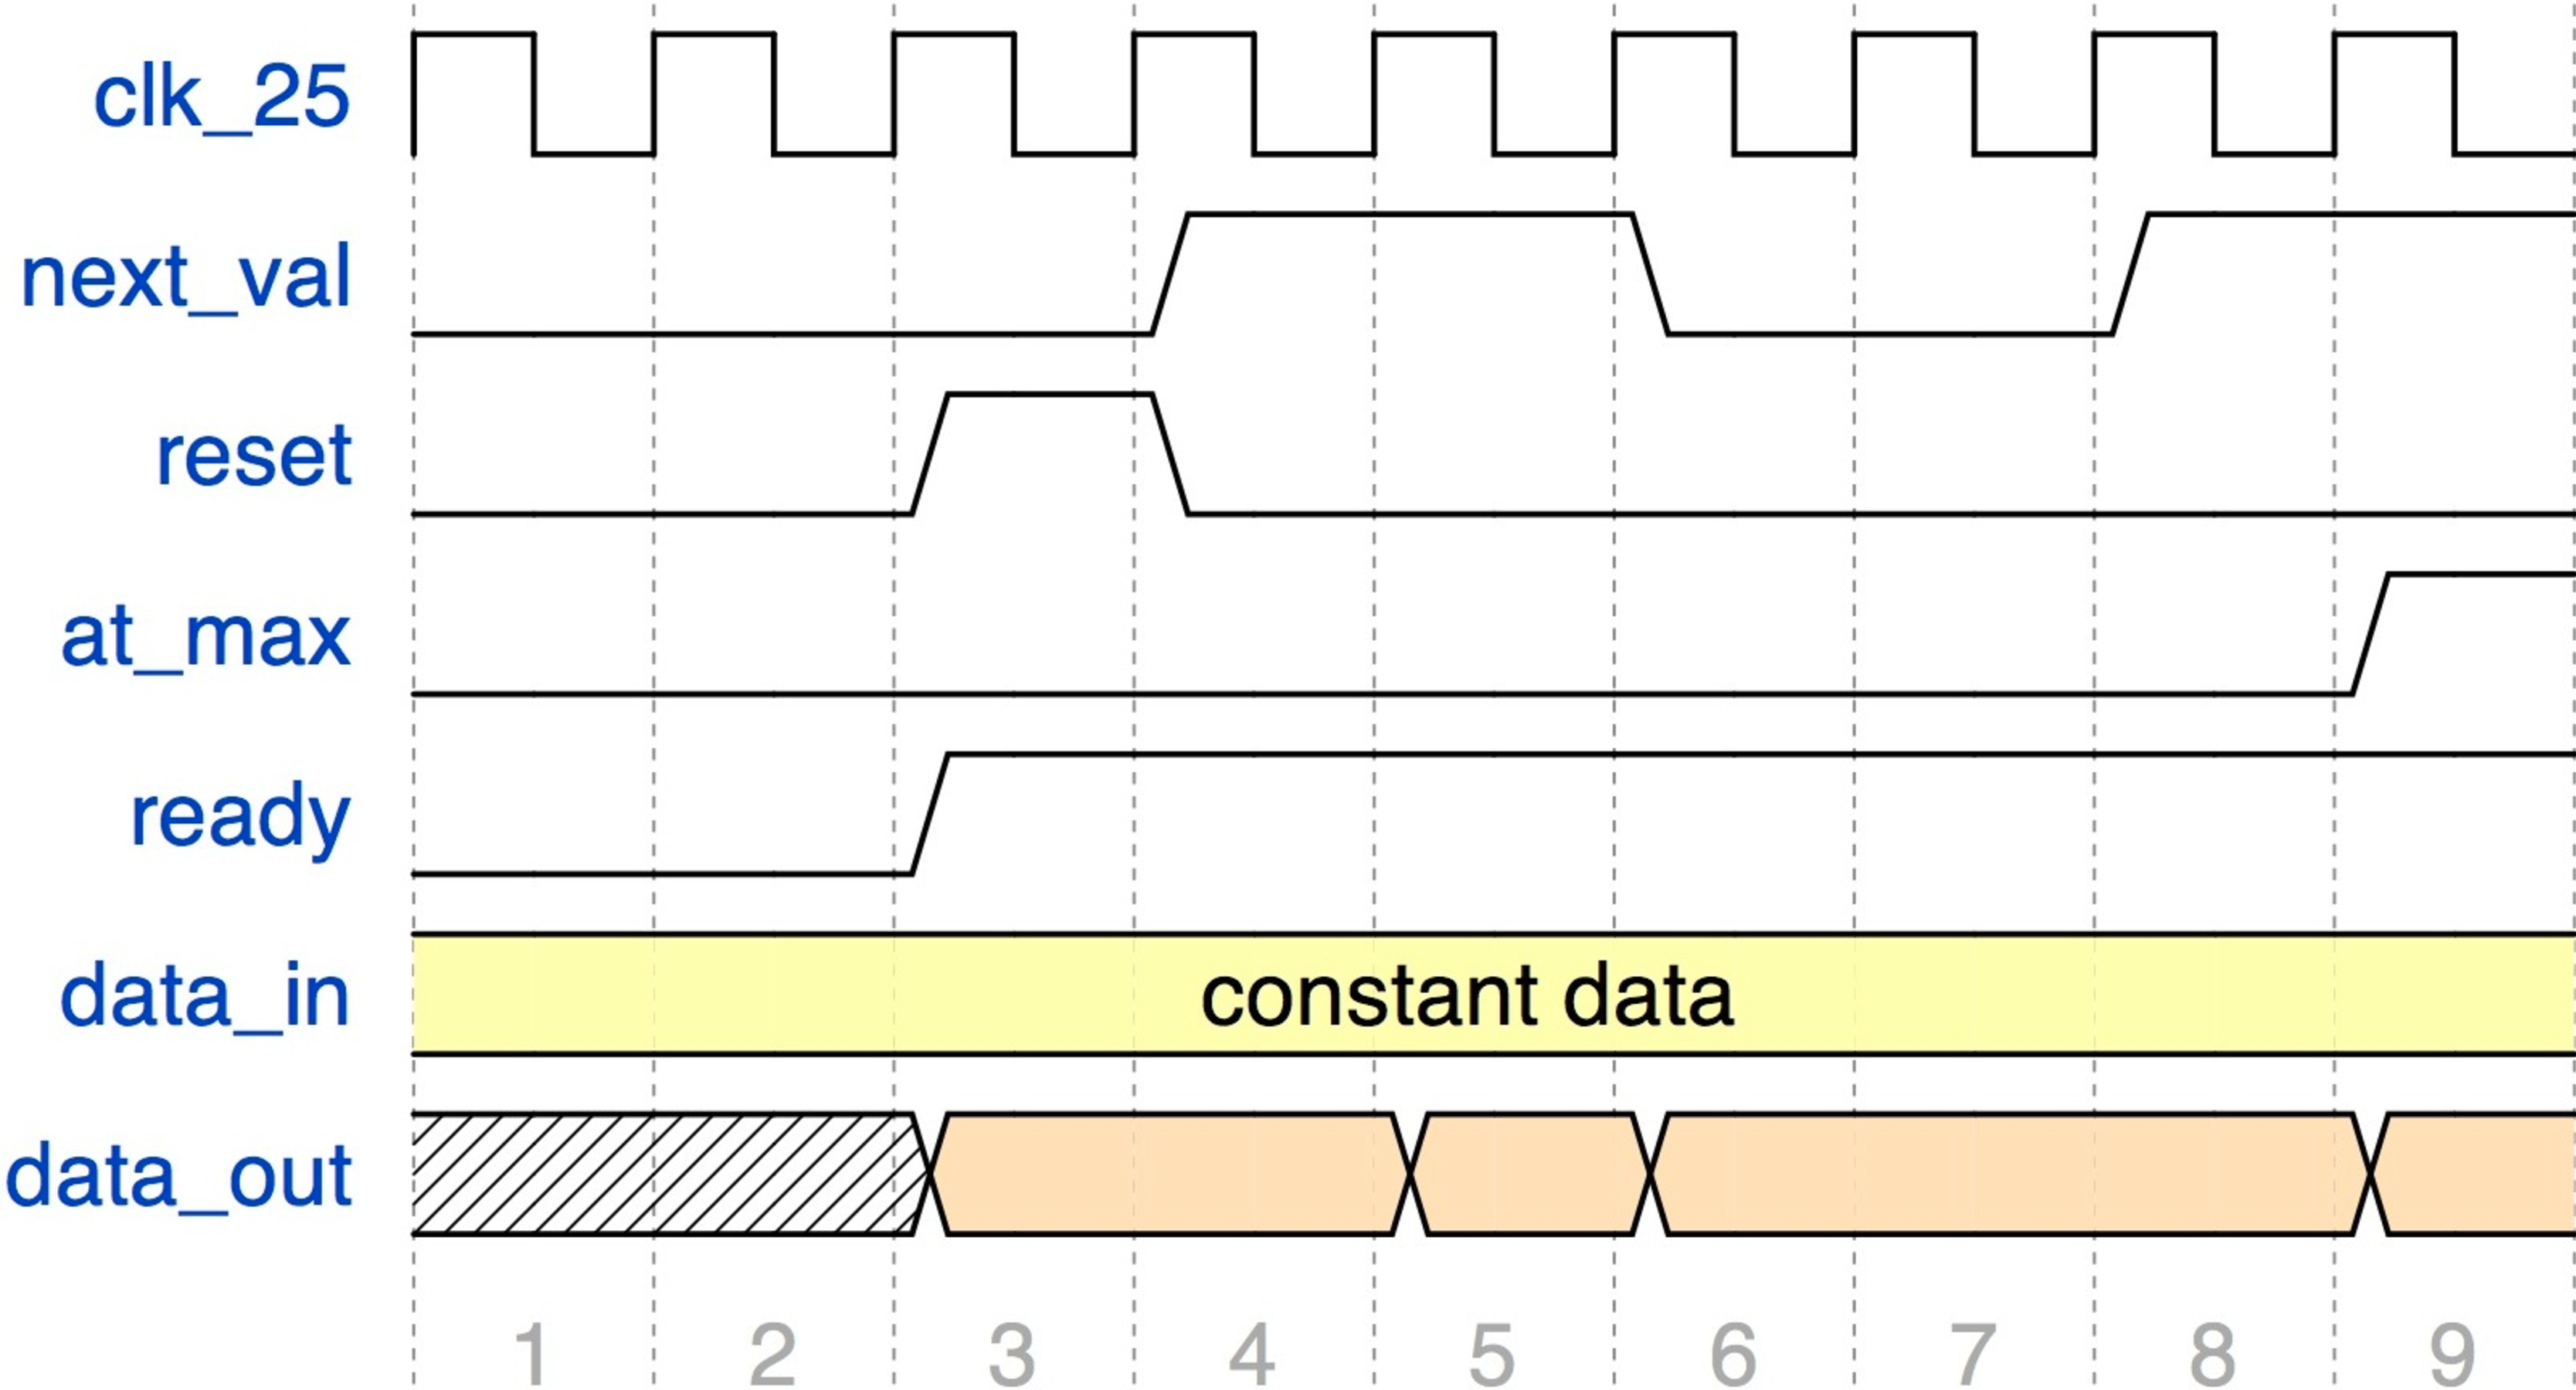
\includegraphics[width=200pt]{timing_diagrams/diff_counter.pdf}
  \caption{Timing diagram of the differential counter}
\end{figure}

In the window generator, the differential counters are hooked up in
such a way that the points are cycled through from left to right down
the screen.

\begin{figure}[H]
  \centering
    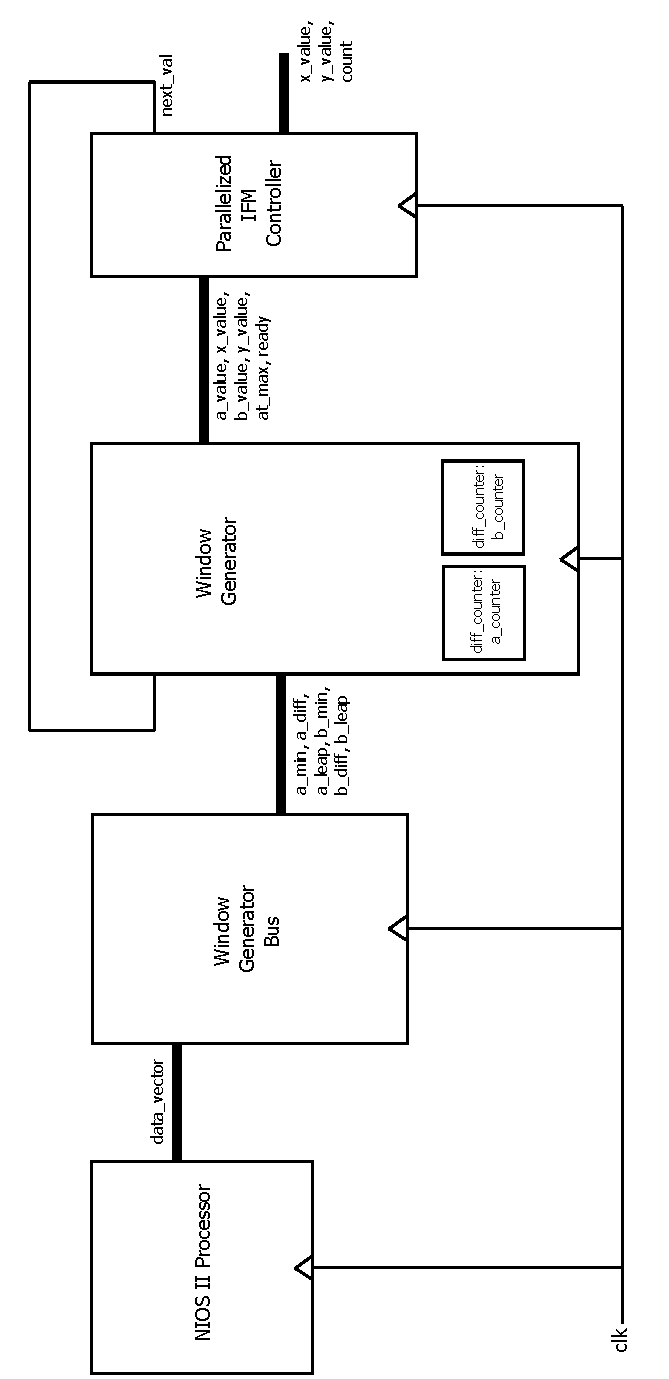
\includegraphics[width=150pt, angle=270]{block_diagrams/win_gen_interior.pdf}
  \caption{Block diagram illustrating $(x, y, a, b)$ tuple dataflow.}
\end{figure}

The window generator takes reset signals from the bus connected to the
NIOS processor. When the window generator is ready for computation
(the same cycle that it is reset by the bus), it asserts a data flag.
When the IFM reads an $(x, y, a, b)$ tuple, it asserts a next value
signal indicating that it will need new data in the following
cycle. Once the window generator runs out of values to give, it
asserts an at max flag.

\begin{figure}[H]
  \centering
    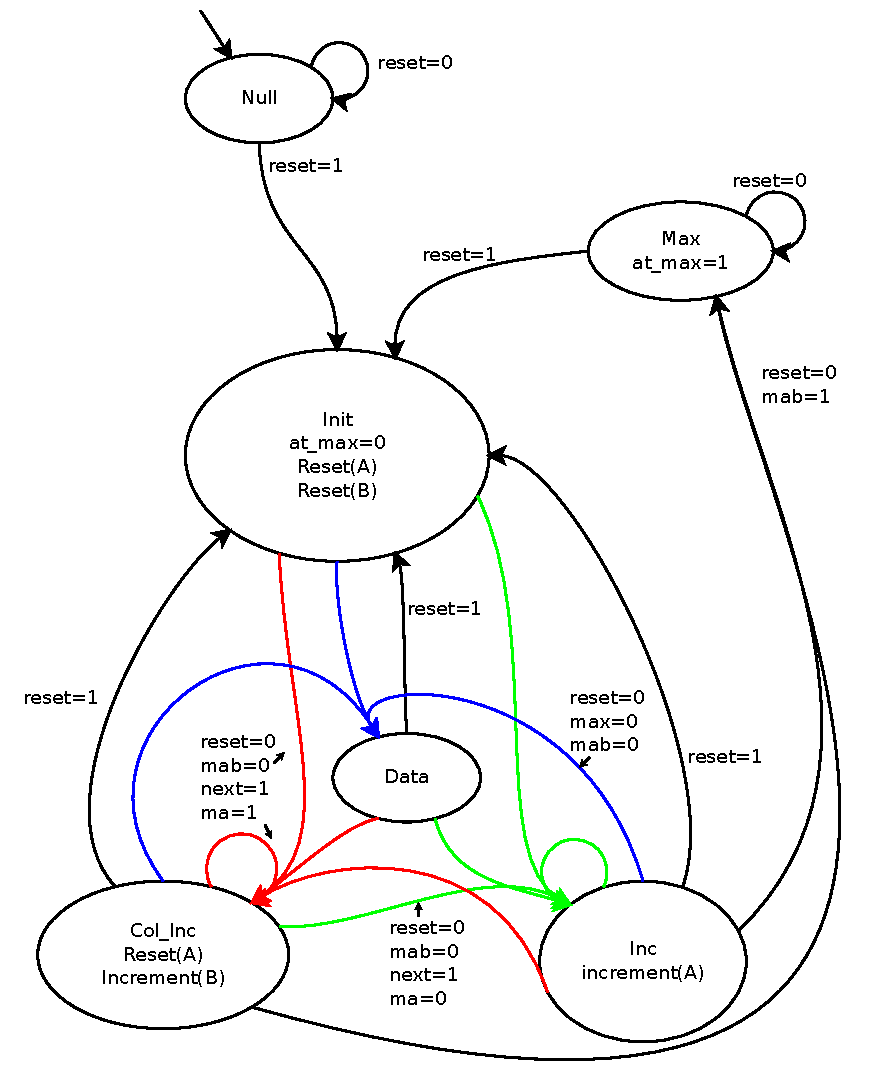
\includegraphics[width=180pt]{state_diagrams/diff_window_gen.pdf}
  \caption{State Diagram for the window generator code, Moore machine:
    signals \texttt{max=c\_cuis=max\_itr},
    \texttt{leap=iter\_count=v\_leap}. Omit unused signals (X) for
    compactness.}
\end{figure}


\begin{figure}[H]
  \centering
    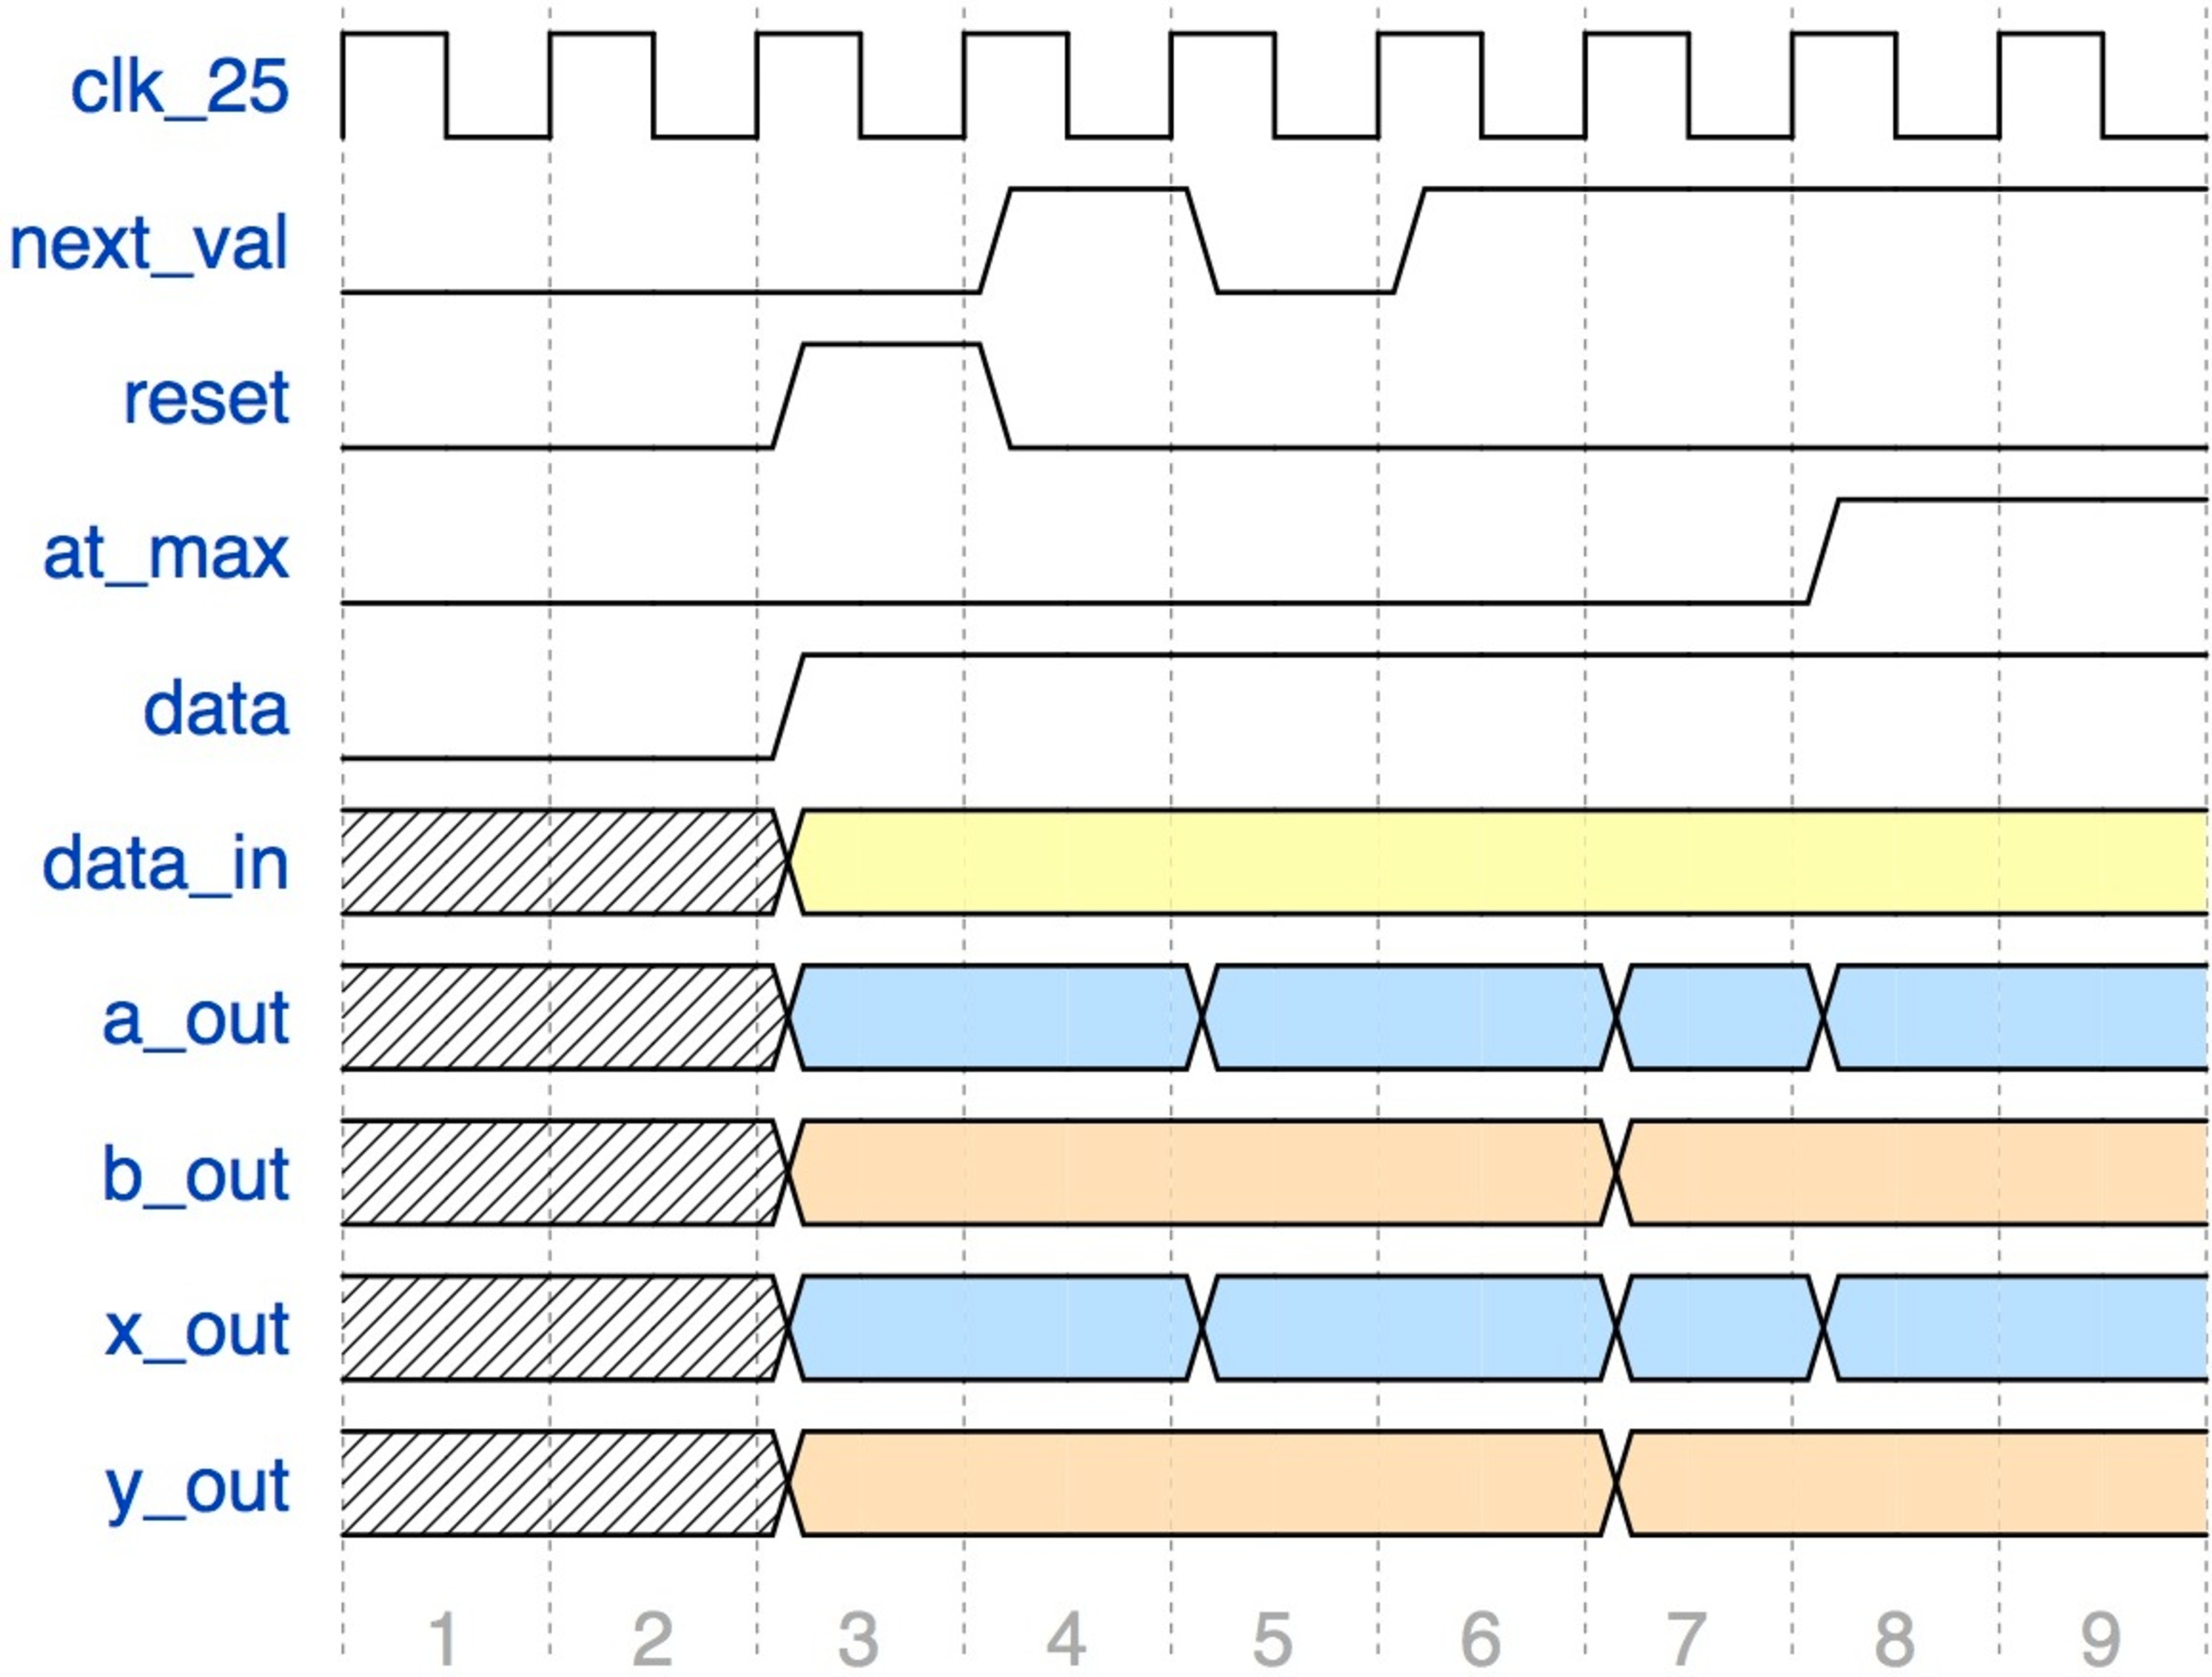
\includegraphics[width=160pt]{timing_diagrams/gen_ifm.pdf}
  \caption{Timing diagram of interface between the window generator
    and the IFMs.}
\end{figure}

\subsection{Parallel IFM Control Module}

Rendering Julia set fractals requires many iterations of relatively
simple computations in the complex plane. This sequence of
computations is independent for each point in the image, which is why
the calculation of fractal sets lends itself to parallel
computation. However, the very nature of the iterated fractal
calculation means that the amount of time spent performing
computations on each individual point can vary drastically,
introducing synchronization issues. It is the responsibility of the
IFM control module to resolve these issues.

\begin{figure}[htb]
  \centering
    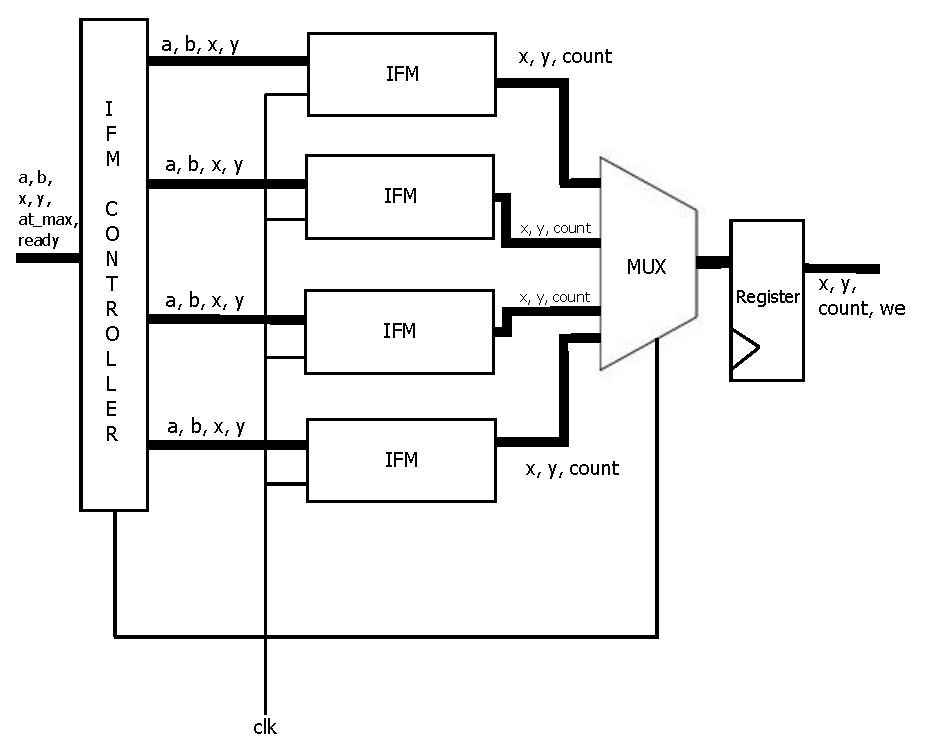
\includegraphics[width=160pt]{block_diagrams/ifmunit.pdf}
  \caption{Block diagram for the IFM wrappers}
\end{figure}


The IFM control module constantly transmits the $(x, y, a, b)$ tuple
currently being expressed by the window generator to each of the
IFMs. When an IFM indicates that it is in the ready state, the
controller asserts a signal instructing the IFM to accept the new data
and begin computation (assuming that the window generator is asserting
the valid data flag).  Simultaneously, the controller signals to the
window generator that it needs the next data tuple in the window. If
more than one IFM is in the ready state at once, the controller only
sends the read and compute signal to one, saving the upcoming data
tuples for the rest.


% ----------------------------------------
\subsection{Iterative Function Module (IFM)}

A quadratic polynomial Julia set is generated by applying the function

\begin{equation}
f(z) = z^2 + c
\end{equation}

repeatedly, where $z,c \in \mathbb{C}$. For any given pair $(z, c)$,
this recurrence will result in one of two outcomes:
\begin{itemize}
\item The magnitude of the complex values generated by the recurrence
  may stay bounded by $2$
\item The magnitude may become unbounded and escape toward infinity
\end{itemize}

A point $z$ on the complex plane is in the Julia set uniquely defined
by the complex number $c$ if and only if the recurrence remains
bounded for $(z, c)$. To determine whether or not a point remains
bounded for a given $c$, we compute a fixed number of iterations on
the recurrence (in our case 127) and report the iteration in which the
value generated has a squared magnitude of greater than $4$. Those
points that do not become unbounded in this many iterations are
considered to be part of the set.

Because the factors of the multiplication are complex numbers,
computing their product involves 3 real-number multiplications. For $z
= a + bi$ we compute\\

\begin{eqnarray}
P_A &=& a^2 \nonumber \\
P_B &=& b^2 \nonumber \\
P_C &=& ab \nonumber
\end{eqnarray}

With these values we can compute:

\begin{eqnarray}
a_{next} &=& P_A - P_B + c_{real}\nonumber \\
b_{next} &=& 2P_C - c_{img} \nonumber \\
|z|^2 &=& P_A + P_B \nonumber 
\end{eqnarray}

The squaring operations for $P_A$ and $P_B$ can be perfomed by a
specialized logical circuit provided as an Altera Megafunction. The
multiplication $P_C$ should be perfomed by embedded multipliers on the
DE2.

\begin{figure}[H]
  \centering
    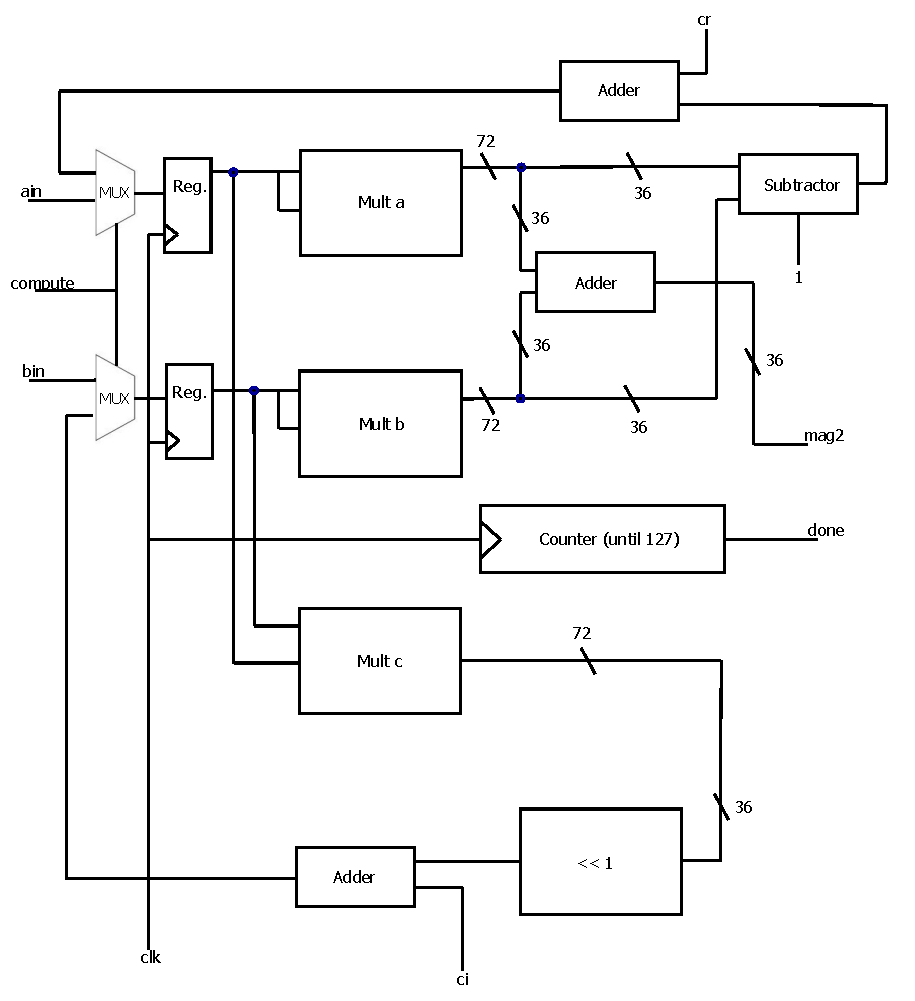
\includegraphics[width=160pt]{block_diagrams/ifm.pdf}
  \caption{Arithmetic Logic Circuit within each IFM}
\end{figure}

Numbers are represented as two's-complement fixed-point binary
values. We restrict ourselves to 36 bits, as the onboard multipliers
are sized as such. In order to accomodate the largest-magnitude value we
expect to come across during any iteration, we require 6 bits to the
left of the radix. Thus, our fixed-point values have 30 bits to the
right of the radix.

\begin{figure}[H]
  \centering
    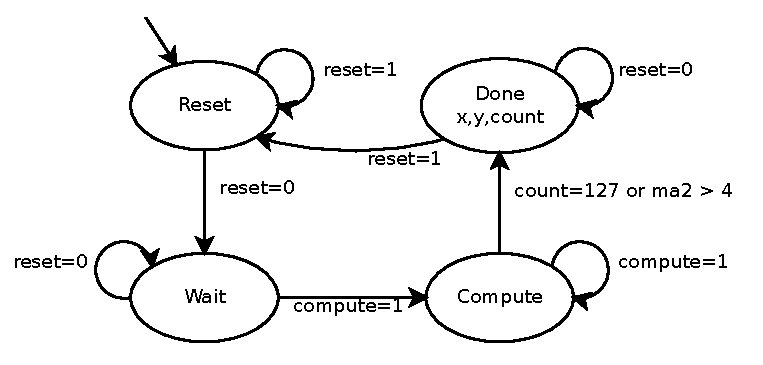
\includegraphics[width=200pt]{state_diagrams/ifm.pdf}
  \caption{State diagram for a single IFM. Moore
    machine: using abstract transition descriptions. Omits unused
    signals for compactness.}
\end{figure}


To more easily facilitate communication with the IFM controller, each
IFM is contained within a wrapper module.  Thus, the IFM controller
need only alter the state of the wrapper module, and the wrapper
module will transmit the signals to the IFMs indicating the desired
behavior.

\begin{figure}[H]
  \centering
    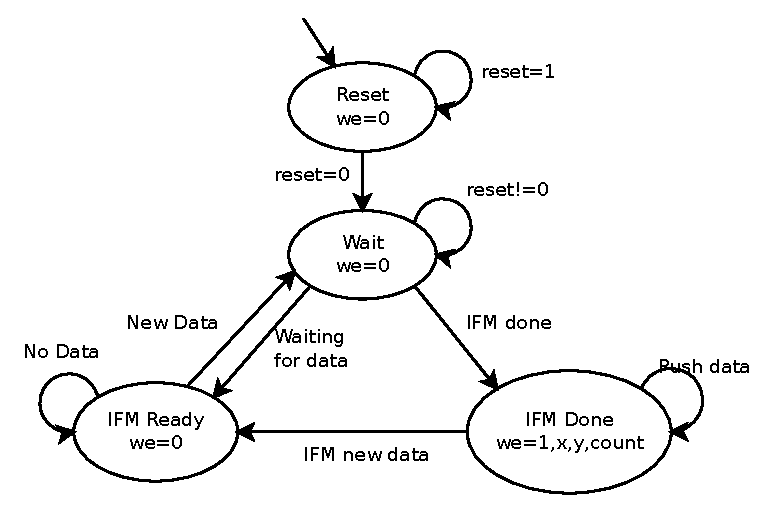
\includegraphics[width=200pt]{state_diagrams/ifmunit.pdf}
  \caption{State diagram for a single IFM unit (IFM handler/wrapper),
    Moore machine: using abstract transition descriptions.}
\end{figure}

If a wrapper module is in the done state, the controller indicates
that its $(x, y, c)$ triple should be read into the output
register. If multiple IFM wrappers are in the done state
simultaneously, the controller chooses one at a time to be read
in. These triples are then augmented with an asserted write enable
flag to indicate that they represent valid data, and should be written
to the Coordinate-Breakaway lookup table.


% ----------------------------------------
\subsection{Coordinate-Breakaway Lookup Table}

After the count associated with each pixel is calculated, it must be
stored in a framebuffer that interfaces both with the Parallel IFM
Control Module as well as the VGA module.

\begin{figure}[H]
  \centering
    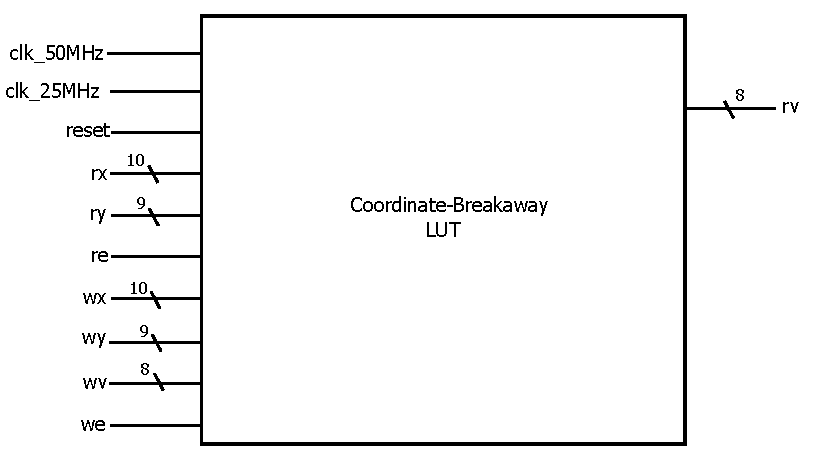
\includegraphics[width=160pt]{block_diagrams/clut.pdf}
  \caption{Block Diagram of the Coordinate-Breakaway LUT: signals on
    the right side are inputs, signals on the left are outputs.}
\end{figure}

For this, we use the SRAM chip that is built into the DE2 board, for
its relatively expansive memory size (versus on-chip memory), fast
speed, and ease of use (versus the SDRAM chip). The SRAM chip has a 
512kibibytes capacity that can be accessed and written to in half a 50MHz
clock cycle, making it ideal for our purposes.

Since we display a $640\times 480$ image in the VGA module and keep 8
bits of iteration information for each pixel, we need a grand total of
300kibibytes to store the information, fitting well within the
confines of the given 512kibibyte SRAM chip.

We use a straightforward addressing scheme to store the count
information, using the $y$ position as the top 9 bits of the address,
and the $x$ position as the bottom 10 bits of the address. This way,
finding the address from a given pixel position is very fast.

A small wrinkle is the fact the SRAM is in fact a 256Kx16 bit memory,
reading and writing in 16 bit chunks. This merely means that the very
bottom bit of the $x$ position does not go to the address, but is
routed to the bitmask signal indicating whether the byte sought is in
the upper or lower half.  Of the 16-bit word that is addressed by the
remaining 18 bits.

\subsection{Reading/Writing}

Since the SRAM has only one IO port, reads and writes must be time
multiplexed. The VGA module will be consistently requesting data from
the SRAM at 25MHz. However, while the fractal is being generated, the
IFMs will be providing information that must be written to the SRAM at
the same frequency. This means that we must interleave reads and
writes to the SRAM.

We can use the structure of the reads from the VGA to our advantage to
make room for the necessary writes. Reads always follow a pattern,
where if we read the lower half of a 16bit word, then we will read the
higher half in the next 25MHz clock cycle. Hence, when we require the
lower half of a word, we can fetch the entire word in one read, save
the higher half in a register, and return it when it's required in the
next clock cycle. In this way, we reduce the frequency of VGA reads
from the SRAM to every other cycle on a 25MHz clock.

\begin{figure}[H]
  \centering
    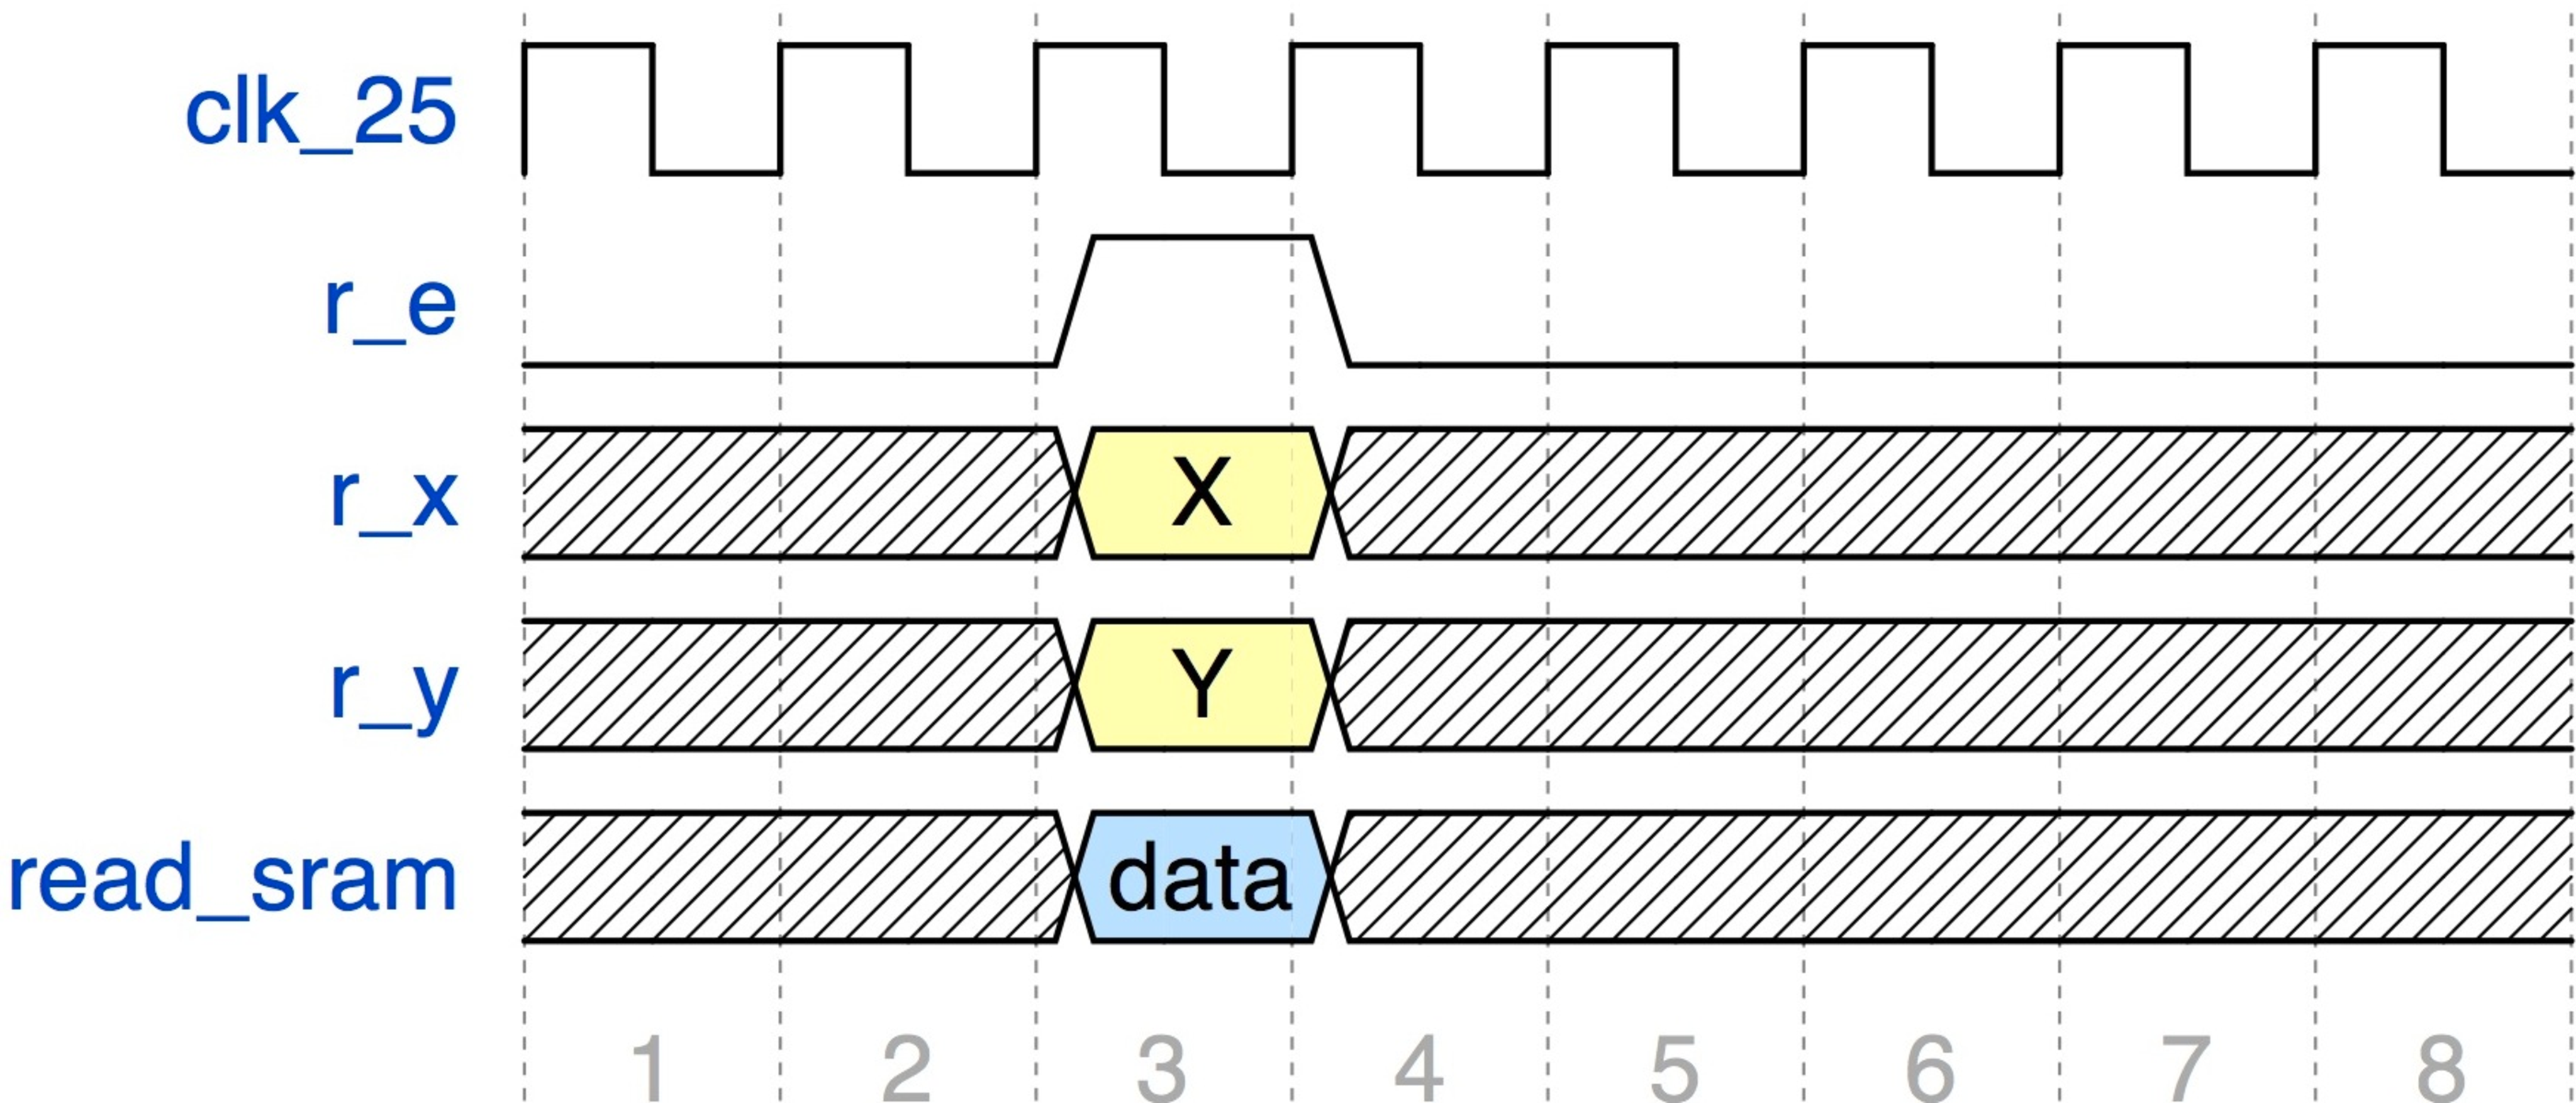
\includegraphics[width=200pt]{timing_diagrams/clut_vga.pdf}
  \caption{Timing diagram of the interface between the
    Coordinate-Breakaway LUT and VGA module}
\end{figure}

Even with every other 25Mhz cycle being dedicated to writing the data
being sent out by the IFMs, the SRAM might still miss a coordinate if
the IFMs are generating their maximum possible throughput of
25MB/s. To account for this, we put the junction serving writedata to
the SRAM on a 50MHz clock. This junction consists of a shift register
that constantly reads from the IFM output, but only shifts when the
SRAM's read enable signal is not being asserted.

\begin{figure}[H]
  \centering 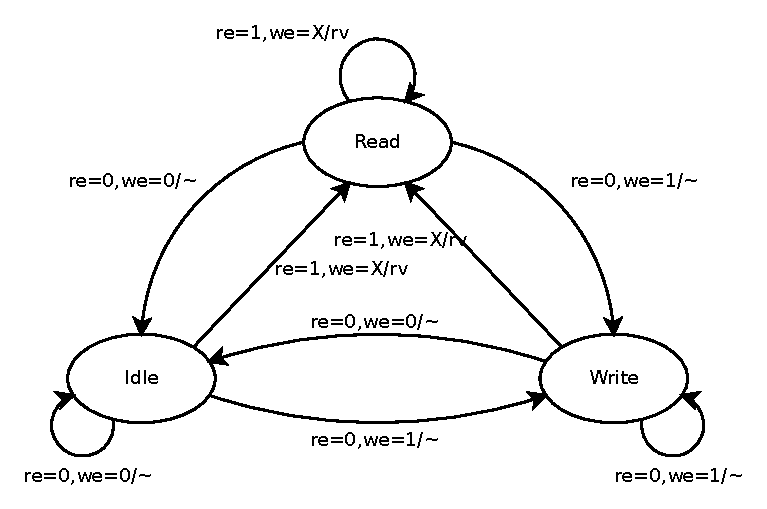
\includegraphics[width=200pt]{state_diagrams/clut.pdf}
  \caption{Simplified State Diagram of the Coordinate-Breakaway LUT:
    Mealy machine, only includes re and we as inputs and rv as an
    output, with $\thicksim$ denoting a lack of outputs}
\end{figure}

This means that a given tuple $(x_j, y_j, c_j, we_j)$ being output by
the IFM controller will be overwritten by the following $(x_k, y_k,
c_k, we_k)$ output during every VGA read cycle. However, since the
shift register is reading from a 25MHz process at 50MHz, it is
guaranteed that every write tuple will be read into the shift register
twice. Because the IFM and VGA controllers are synchronized, the VGA
read always occurs when $j \neq k$. But because every tuple is read
into the shift register twice, the value that was overwritten, $(x_j,
y_j, c_j, we_j)$, must also exist in the next cell over, guaranteeing
reliable data transmission.

\begin{figure}[H]
  \centering
  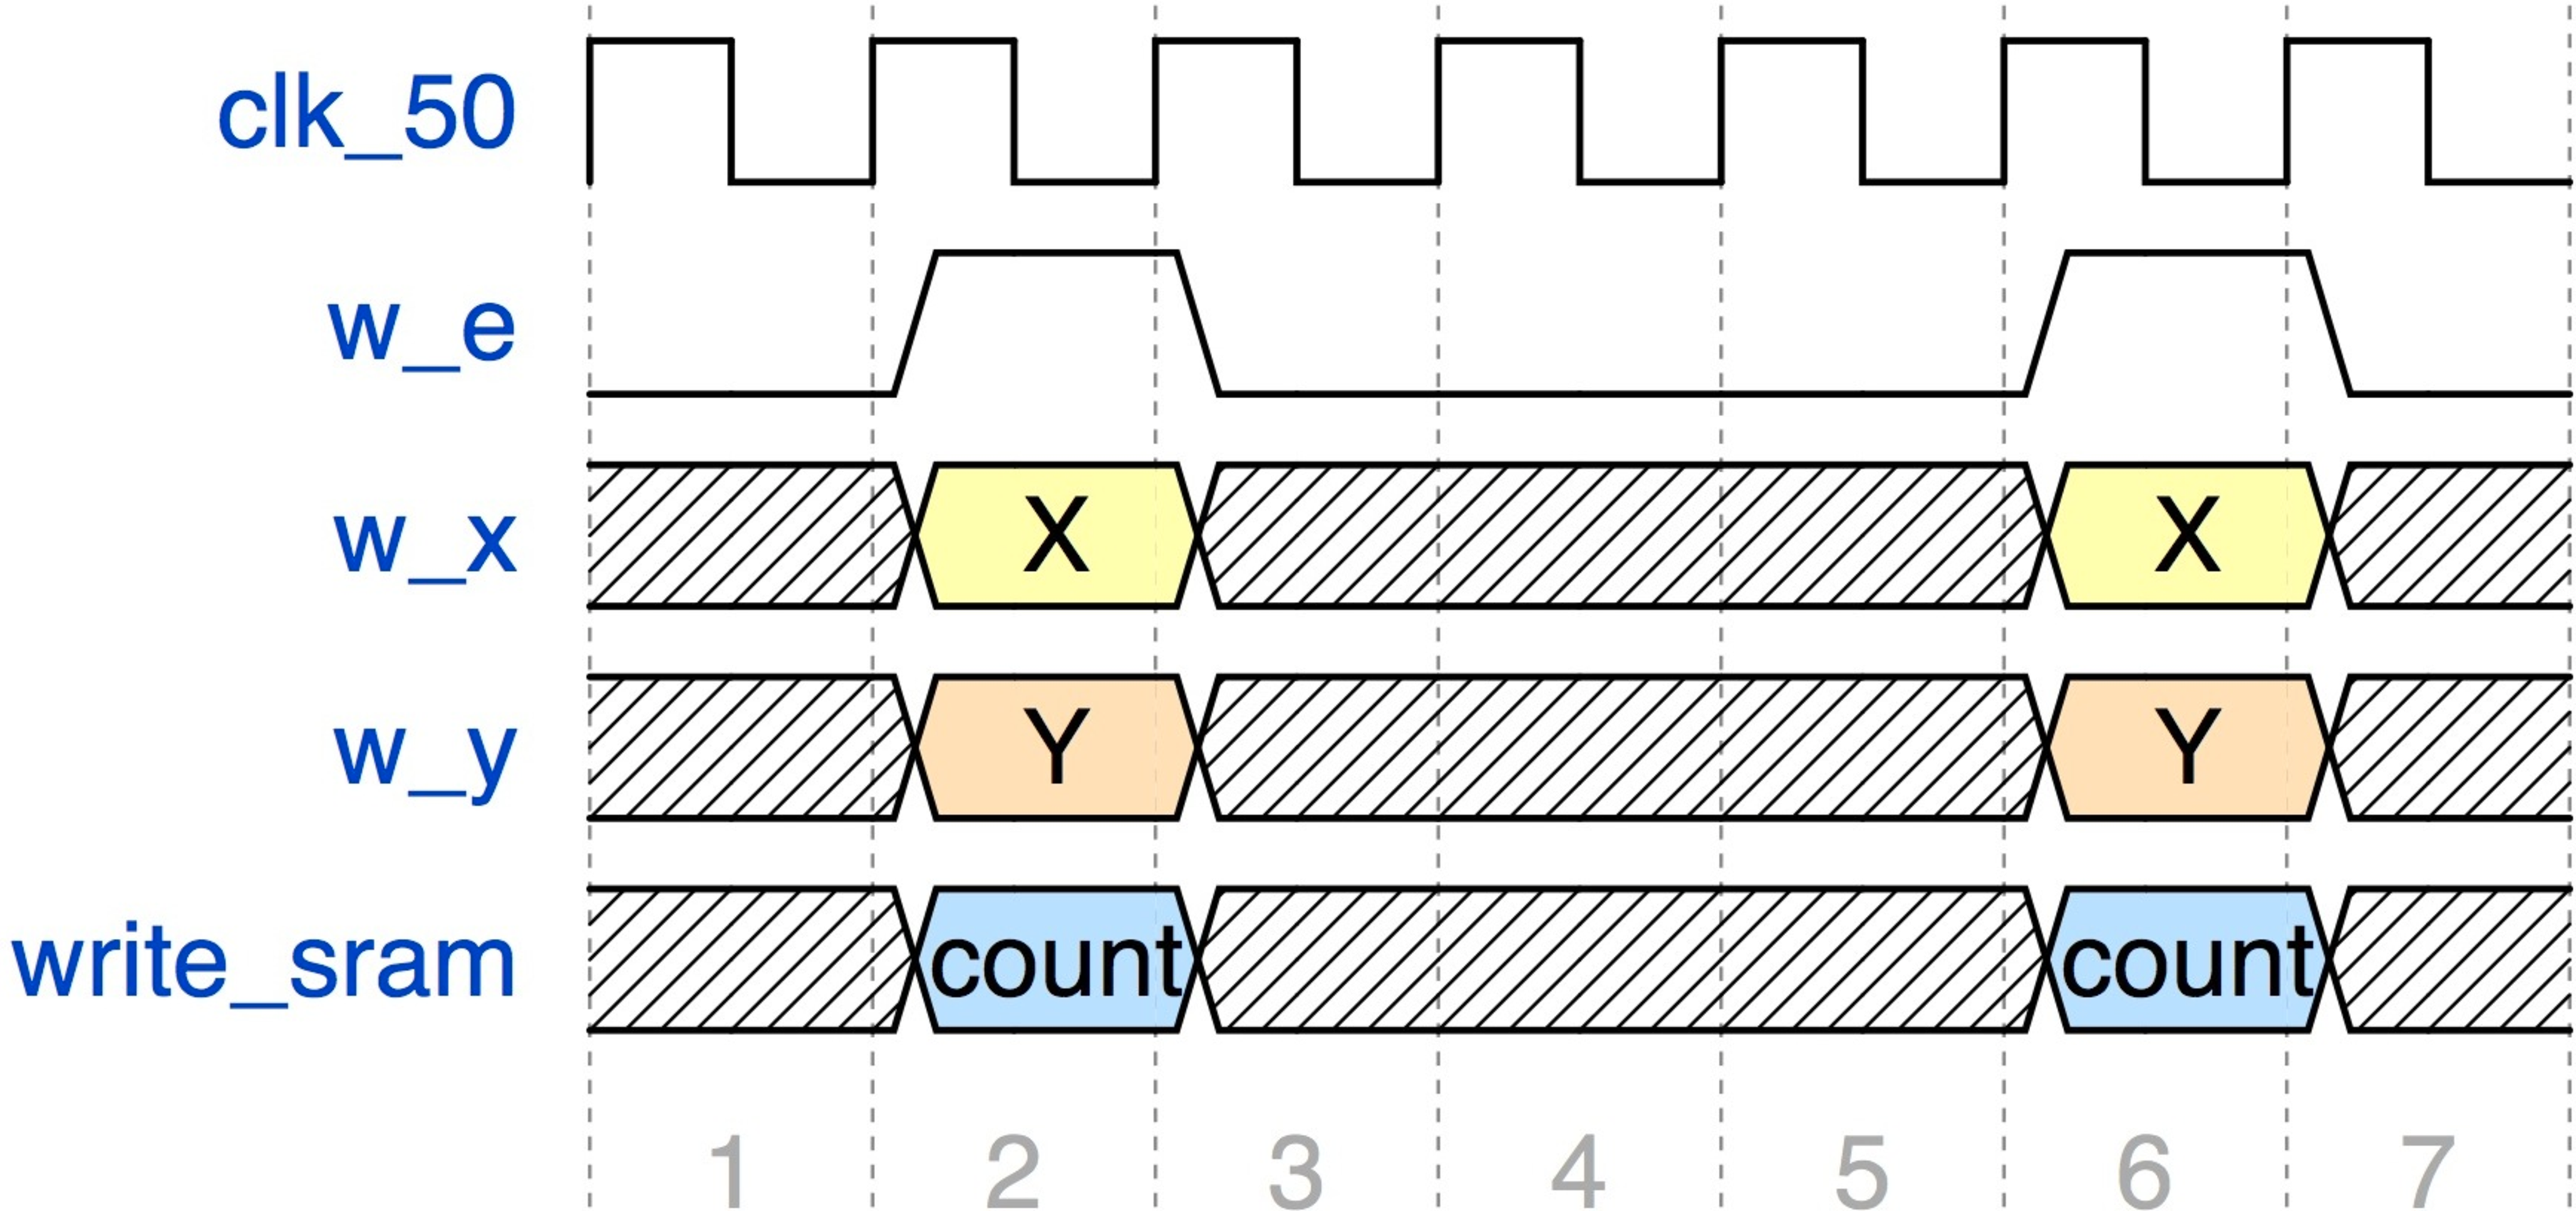
\includegraphics[width=200pt]{timing_diagrams/ifm_clut.pdf}
  \caption{Timing diagram of the interface between the IFMs and the
    Coordinate-Breakaway LUT.}
\end{figure}

Dangerous though it may be, the effect of having a faster clock for
the SRAM write junction is well contained.  No processes depend on the
state of the write junction, and the junction is free to produce
redundant write data without consequence. The write junction merely
serves as a conduit through which writedata is transmitted.


\subsection{VGA Module}

In order to display the generated Julia set, we connect a VGA
controller to the Coordinate-Breakaway lookup table. As the controller
cycles through output coordinates within the display area, it modifies
the read address signal for the lookup table. The data signal coming
from the RAM is thus the breakaway value associated with that
coordinate.

\begin{figure}[H]
  \centering 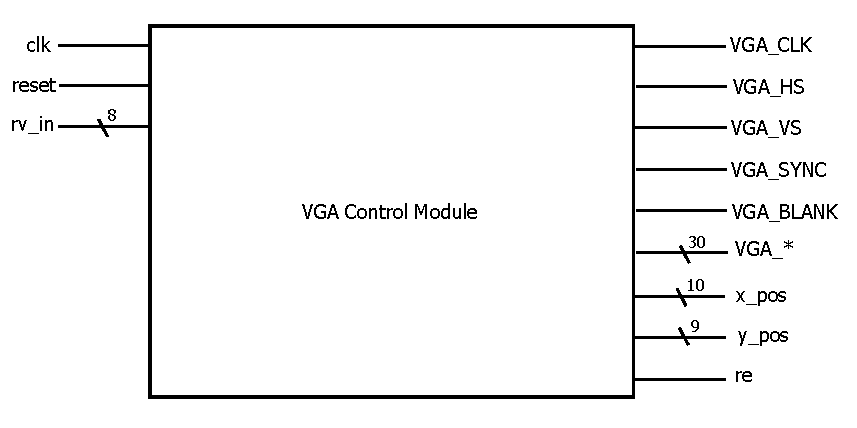
\includegraphics[width=200pt]{block_diagrams/vga.pdf}
  \caption{Block diagram of the VGA module}
\end{figure}

This breakaway value is passed through a decoder known as the
Colorization Lookup Table and the resulting $(R, G, B)$ signal tuple
is sent to the VGA port.

% ----------------------------------------
% figures for the VGA


\begin{figure}[H]
  \centering 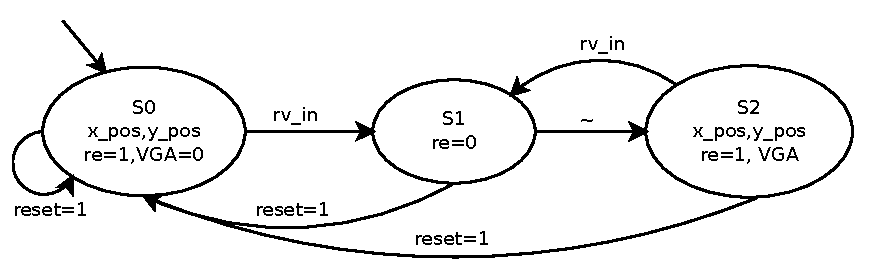
\includegraphics[width=200px]{state_diagrams/vga.pdf}
  \caption{State diagram for the \texttt{VGA} module, Mealy machine:
    $\thicksim$ stands in for no input/output, and VGA stands in for
    all the VGA\_ signals (\texttt{VGA\_CLK}, \texttt{VGA\_HS},
    \texttt{VGA\_VS}, \texttt{VGA\_BLANK}, \texttt{VGA\_SYNC},
    \texttt{VGA\_R}, \texttt{VGA\_G}, \texttt{VGA\_B}). Omits unused
    signals for compactness.}
\end{figure}


% ------------------------------------------------------------
\section{Parametrization Modules}

These modules might be used parameterize the output fractal

\begin{itemize}
\item PS/2 Keyboard input can be used to allow the user to specify
  fractal recomputation using a different set of parameters,
  permitting the modification of window ranges and Julia Set
  constants. Keyboard input would be facilitated through the Nios II
  processor and would require a reexecution of the Window Generator.
\item We could create a module for permuting the display colors given
  by the Colorization Lookup table using a periodic function, thus
  causing the colors to cycle. This module would allow us to modify
  the way the fractal looks without recomputing it.
\item Spectral analysis module takes audio input and uses it to
  influence the behavior of the Color Permutation module.
\end{itemize}


% ------------------------------------------------------------
% !!! UPDATE MILESTONES IF NECESSARY
\section{Updated Milestones}

\begin{itemize}
\item Milestone 1 (Mar 27): \\ Develop a Window Generator and
  Parallelized IFM module that can communicate successfully.
\item Milestone 2 (Apr 10): \\ Display the colorized (and static)
  Julia set through VGA.
\item Milestone 3 (Apr 24): \\ Implement parameter mutation, with
  subsequent updates to the displayed Julia set.
\item Final Report and Presentation (May 10)
\end{itemize}

\end{document}
